% Options for packages loaded elsewhere
\PassOptionsToPackage{unicode}{hyperref}
\PassOptionsToPackage{hyphens}{url}
\PassOptionsToPackage{dvipsnames,svgnames,x11names}{xcolor}
%
\documentclass[
  12pt]{article}

\usepackage{amsmath,amssymb}
\usepackage{iftex}
\ifPDFTeX
  \usepackage[T1]{fontenc}
  \usepackage[utf8]{inputenc}
  \usepackage{textcomp} % provide euro and other symbols
\else % if luatex or xetex
  \usepackage{unicode-math}
  \defaultfontfeatures{Scale=MatchLowercase}
  \defaultfontfeatures[\rmfamily]{Ligatures=TeX,Scale=1}
\fi
\usepackage{lmodern}
\ifPDFTeX\else  
    % xetex/luatex font selection
\fi
% Use upquote if available, for straight quotes in verbatim environments
\IfFileExists{upquote.sty}{\usepackage{upquote}}{}
\IfFileExists{microtype.sty}{% use microtype if available
  \usepackage[]{microtype}
  \UseMicrotypeSet[protrusion]{basicmath} % disable protrusion for tt fonts
}{}
\makeatletter
\@ifundefined{KOMAClassName}{% if non-KOMA class
  \IfFileExists{parskip.sty}{%
    \usepackage{parskip}
  }{% else
    \setlength{\parindent}{0pt}
    \setlength{\parskip}{6pt plus 2pt minus 1pt}}
}{% if KOMA class
  \KOMAoptions{parskip=half}}
\makeatother
\usepackage{xcolor}
\setlength{\emergencystretch}{3em} % prevent overfull lines
\setcounter{secnumdepth}{5}
% Make \paragraph and \subparagraph free-standing
\makeatletter
\ifx\paragraph\undefined\else
  \let\oldparagraph\paragraph
  \renewcommand{\paragraph}{
    \@ifstar
      \xxxParagraphStar
      \xxxParagraphNoStar
  }
  \newcommand{\xxxParagraphStar}[1]{\oldparagraph*{#1}\mbox{}}
  \newcommand{\xxxParagraphNoStar}[1]{\oldparagraph{#1}\mbox{}}
\fi
\ifx\subparagraph\undefined\else
  \let\oldsubparagraph\subparagraph
  \renewcommand{\subparagraph}{
    \@ifstar
      \xxxSubParagraphStar
      \xxxSubParagraphNoStar
  }
  \newcommand{\xxxSubParagraphStar}[1]{\oldsubparagraph*{#1}\mbox{}}
  \newcommand{\xxxSubParagraphNoStar}[1]{\oldsubparagraph{#1}\mbox{}}
\fi
\makeatother


\providecommand{\tightlist}{%
  \setlength{\itemsep}{0pt}\setlength{\parskip}{0pt}}\usepackage{longtable,booktabs,array}
\usepackage{calc} % for calculating minipage widths
% Correct order of tables after \paragraph or \subparagraph
\usepackage{etoolbox}
\makeatletter
\patchcmd\longtable{\par}{\if@noskipsec\mbox{}\fi\par}{}{}
\makeatother
% Allow footnotes in longtable head/foot
\IfFileExists{footnotehyper.sty}{\usepackage{footnotehyper}}{\usepackage{footnote}}
\makesavenoteenv{longtable}
\usepackage{graphicx}
\makeatletter
\def\maxwidth{\ifdim\Gin@nat@width>\linewidth\linewidth\else\Gin@nat@width\fi}
\def\maxheight{\ifdim\Gin@nat@height>\textheight\textheight\else\Gin@nat@height\fi}
\makeatother
% Scale images if necessary, so that they will not overflow the page
% margins by default, and it is still possible to overwrite the defaults
% using explicit options in \includegraphics[width, height, ...]{}
\setkeys{Gin}{width=\maxwidth,height=\maxheight,keepaspectratio}
% Set default figure placement to htbp
\makeatletter
\def\fps@figure{htbp}
\makeatother

\addtolength{\oddsidemargin}{-.5in}%
\addtolength{\evensidemargin}{-1in}%
\addtolength{\textwidth}{1in}%
\addtolength{\textheight}{1.7in}%
\addtolength{\topmargin}{-1in}%
\makeatletter
\@ifpackageloaded{caption}{}{\usepackage{caption}}
\AtBeginDocument{%
\ifdefined\contentsname
  \renewcommand*\contentsname{Table of contents}
\else
  \newcommand\contentsname{Table of contents}
\fi
\ifdefined\listfigurename
  \renewcommand*\listfigurename{List of Figures}
\else
  \newcommand\listfigurename{List of Figures}
\fi
\ifdefined\listtablename
  \renewcommand*\listtablename{List of Tables}
\else
  \newcommand\listtablename{List of Tables}
\fi
\ifdefined\figurename
  \renewcommand*\figurename{Figure}
\else
  \newcommand\figurename{Figure}
\fi
\ifdefined\tablename
  \renewcommand*\tablename{Table}
\else
  \newcommand\tablename{Table}
\fi
}
\@ifpackageloaded{float}{}{\usepackage{float}}
\floatstyle{ruled}
\@ifundefined{c@chapter}{\newfloat{codelisting}{h}{lop}}{\newfloat{codelisting}{h}{lop}[chapter]}
\floatname{codelisting}{Listing}
\newcommand*\listoflistings{\listof{codelisting}{List of Listings}}
\makeatother
\makeatletter
\makeatother
\makeatletter
\@ifpackageloaded{caption}{}{\usepackage{caption}}
\@ifpackageloaded{subcaption}{}{\usepackage{subcaption}}
\makeatother

\ifLuaTeX
  \usepackage{selnolig}  % disable illegal ligatures
\fi
\usepackage[]{natbib}
\bibliographystyle{agsm}
\usepackage{bookmark}

\IfFileExists{xurl.sty}{\usepackage{xurl}}{} % add URL line breaks if available
\urlstyle{same} % disable monospaced font for URLs
\hypersetup{
  pdftitle={DOGE Days on Reddit: Decoding Public Sentiment in a Federal Shakeup},
  pdfauthor={Kevin Linares; Felix Baez-Santiago; Aria Lu; Gloria Zhou},
  pdfkeywords={Reddit, Federal Government, DOGE},
  colorlinks=true,
  linkcolor={blue},
  filecolor={Maroon},
  citecolor={Blue},
  urlcolor={Blue},
  pdfcreator={LaTeX via pandoc}}



\begin{document}


\def\spacingset#1{\renewcommand{\baselinestretch}%
{#1}\small\normalsize} \spacingset{1}


%%%%%%%%%%%%%%%%%%%%%%%%%%%%%%%%%%%%%%%%%%%%%%%%%%%%%%%%%%%%%%%%%%%%%%%%%%%%%%

\date{March 20, 2025}
\title{\bf DOGE Days on Reddit: Decoding Public Sentiment in a Federal
Shakeup}
\author{
Kevin Linares\\
University of Maryland\\
and\\Felix Baez-Santiago\\
and\\Aria Lu\\
and\\Gloria Zhou\\
University of Michigan\\
}
\maketitle

\bigskip
\bigskip
\begin{abstract}
This study explores the impact of the Department of Government
Efficiency (DOGE)'s federal workforce reductions on public sentiment,
utilizing Reddit as a data source. By scraping and analyzing posts and
comments related to DOGE, we examined public reactions, including fear,
anxiety, and support, during a period of significant governmental
change. The analysis reveals how specific news events influenced online
discourse and highlights the utility of social media for understanding
public perception of policy impacts.
\end{abstract}

\noindent%
{\it Keywords:} Reddit, Federal Government, DOGE
\vfill

\newpage
\spacingset{1.9} % DON'T change the spacing!


\section{Introduction}\label{sec-intro}

Since it's inception in January of 2025, the Department of Government
Efficiency (DOGE) has fired over 200,000 federal workers in an effort by
the new administration to keep a campaign promise in reducing federal
government. However, DOGE's overreaching approach and often illegal
tactics has resulted sparked fear and anxiety among the federal
workforce, thus taking a toll on their mental health. Many are uncertain
about their career faith as it is in the hands of outsiders that
disregard internal policies with no remorse. The current topic on how
DOGE is impacting federal worker's perceptions of job security is likely
to continue and worsen over the next few months, given DOGE's
nontransparent and unconventional methods without accountability. We
propose that Reddit as a platform offers researchers a vantage look into
lively discussions, timely reactions, and grievances from federal
workers on this topic. Furthermore, we also expect to capture positive
reactions to DOGE's approach in reducing the federal workforce.

\section{Methods}\label{sec-meth}

\emph{Search Terms}. Our preliminary Reddit API scrape allowed us to
decide on a set of keyword searches related to this topic of research.
This was an iterative process that resulted in the use of 8 keywords we
used to search for posts related to the topic of interest (see Table 1).
We excluded keywords that were either vague or broad such as ``Elon
Musk'' or ``drain the swamp.'' Additionally, we examined subreddit posts
and found a plethora of unrelated posts using our keyword search list.
For instance, searching for ``Fork in the Road'' brought back several
subreddits on motorcycles and mountain biking. Additionally, searching
for ``DOGE'' also brought back posts on DOGEcoin which is unrelated to
our topic. Therefore, we meticoulsly combed through a list of subreddits
we acquired from our initial scrape and selected those that contaiend
relevant posts. To compensate for balance on this topic, we included
conservative subreddits such as ``neoliberal'', ``AskConservitives'' as
well as we avoided specific agency subreddits, for instance ``NIH'' or
``CDC'' as to not overwhelm one particular view point. Overall we ended
with 19 subreddits (see appendix) and 8 keywords resulting in 152 unique
combinations to scrape.

\begin{longtable}[]{@{}l@{}}
\caption{List of keywords related to topic}\tabularnewline
\toprule\noalign{}
search\_term \\
\midrule\noalign{}
\endfirsthead
\toprule\noalign{}
search\_term \\
\midrule\noalign{}
\endhead
\bottomrule\noalign{}
\endlastfoot
DOGE \\
Department of Government Efficiency \\
wasteful spending \\
government waste \\
government fraud \\
reduction in force \\
rif \\
fork in the road \\
\end{longtable}

\emph{Analytic Plan}. We listened to the Reddit API from March 2 through
the 10th on every top of the hour by scraping each combination of our
seven keywords and 20 subreddits resulting in 152 API hits per hour.
Reddit API scraping limits were managed by setting a sleep timer in
between API hits. As new Reddit posts were scraped they were entered
into a data table without preprocessing. After the listening period, the
accumulated number of unprocessed posts was 643. Every row in our data
table equated to one post, and we had 8 columns to include the date and
time of the post, title and text of post, subreddit where the post
derived from, number of comments associated with it, url, and we
recorded the search term that was used to collect the post. We processed
the posts to exclude duplicates, and in some instance two different
keywords resulted in scraping the same posts so we kept we dropped one
of them. Post text were cleaned in terms of removing weblinks and when
possible translating special character such as the at sign to the word
``at.'' The date column was converted to a date class variable and we
extracted the day of the week and time of day from it to use in
analysis. Cleaning our scraped posts resulted in 557 posts.

A glance at the posts revealed that many of them are factual statements,
questions, or re-postings of news articles and videos. Therefore, these
texts do not lend themselves to be coded for favorability, and we
decided to also scrape the comments associated with each post. This
resulted in 12,553 comments, post processing, containing information
about the score, up/down votes, and date/time posted. We removed
comments that had only a weblink, video, or image as these cannot be
coded. A look into some of these comments revealed more opinionated
statements and reactions which we than randomly (without replacement)
selected 400 comments assigned to four graduate students to code for
whether the comment favored DOGE's approach to the reduction in the
federal force, opposed, or was neutral.

\section{Results}\label{results}

We show the number of posts pre/post processing by day in Figure 1
during the timeframe that we collected these data.. There appears to be
a noticeable peak in activity during the middle of the week. However, we
don't have enough data across weeks to conclusively say it's due to the
day of the week itself. It's more likely that these spikes are linked to
specific events that occurred on those days, which sparked
conversations. The two peaks in our graph could be attributed to two
major news stories. On March 5, Elon Musk made a statement about wanting
to ``save Western civilization from empathy,'' and on March 6, there
were reports that President Trump was limiting Musk's authority due to
backlash over cuts to DOGE. These events likely had a significant impact
on the volume of Reddit posts related to Elon Musk and DOGE, driving the
observed spikes in activity.

On May third, news outlets started reporting that DOGE was claiming
\$105 billion dollars in savings from cutting ``wasteful'' spending by
layoffs and cutting foreign aid. This amount is controversial since
since the receipts shown on their site only amount to less than
\href{https://abcnews.go.com/US/doge-website-now-saved-105-billion-backtracked-earlier/story?id=119408347}{\$9.6
billion}. This could have prompted Reddit users to take to subreddits
and provide their opinion or thoughts on this matter.

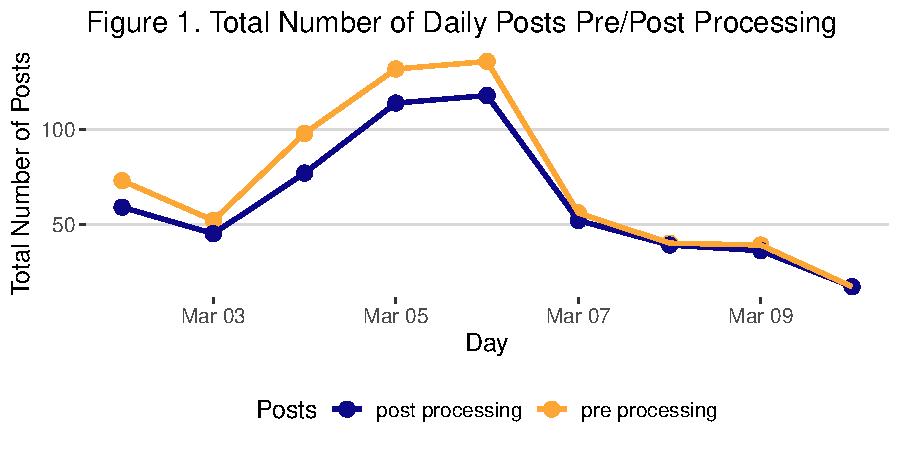
\includegraphics{paper_files/figure-pdf/unnamed-chunk-3-1.pdf}

We see a peak in the comments in Figure 2 during March 6th, which was a
Thursday, and perhaps in anticipation of DOGE policies that often are
released on Friday morning and have come to be known as
``\href{https://smotus.substack.com/p/friday-night-musk-acre}{Musk-acre
Friday}.''

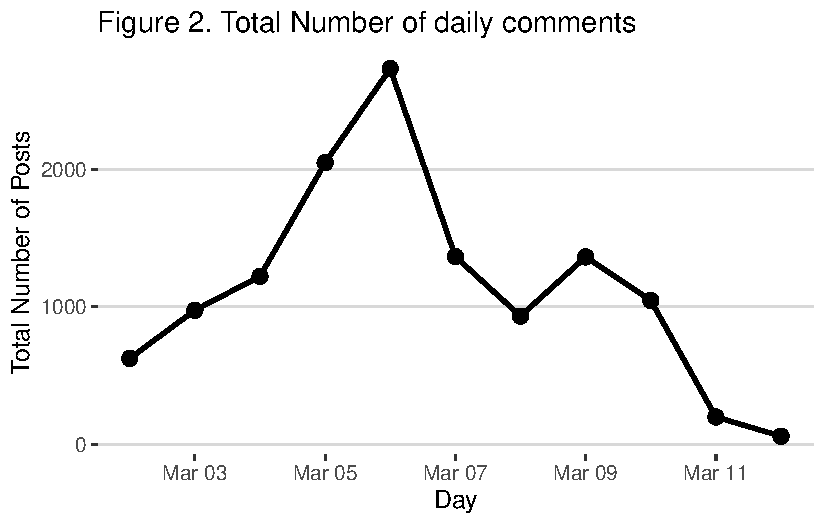
\includegraphics{paper_files/figure-pdf/unnamed-chunk-4-1.pdf}

Most posts occur during the early morning, noon, and afternoon hours
(see Figure 3). The highest peak is around lunchtime, likely due to
people posting during their lunch break. There is also significant
activity in the afternoon, evening, and early morning. This could be
because people have more free time or stay up late, allowing them to
take the time to write posts, which require more effort than quick
interactions. The fewest posts are seen in the morning, which makes
sense as people are typically getting ready for work, commuting, or
sleeping in. The trend for comments (see Figure 4) mirrors that of
posts. This makes sense because people are likely using Reddit at
similar times for both posting and commenting. However, the volume of
comments is much higher than the number of posts, as each post receives
many comments from different users.

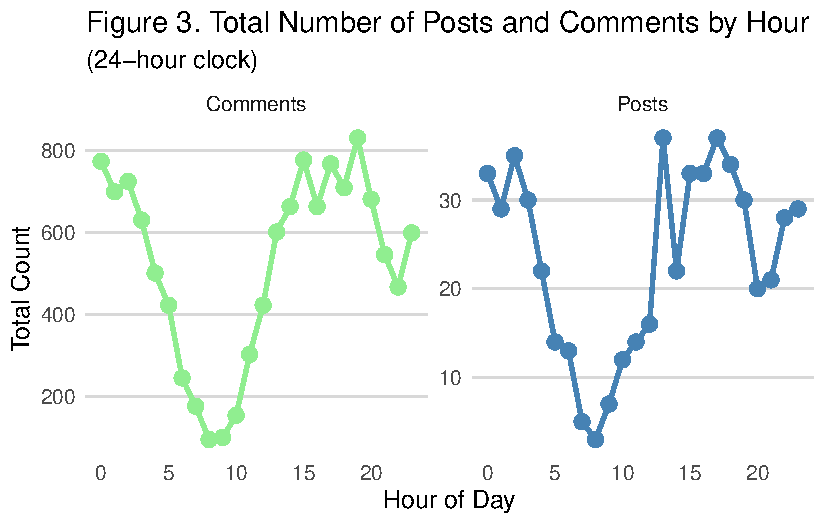
\includegraphics{paper_files/figure-pdf/unnamed-chunk-5-1.pdf}

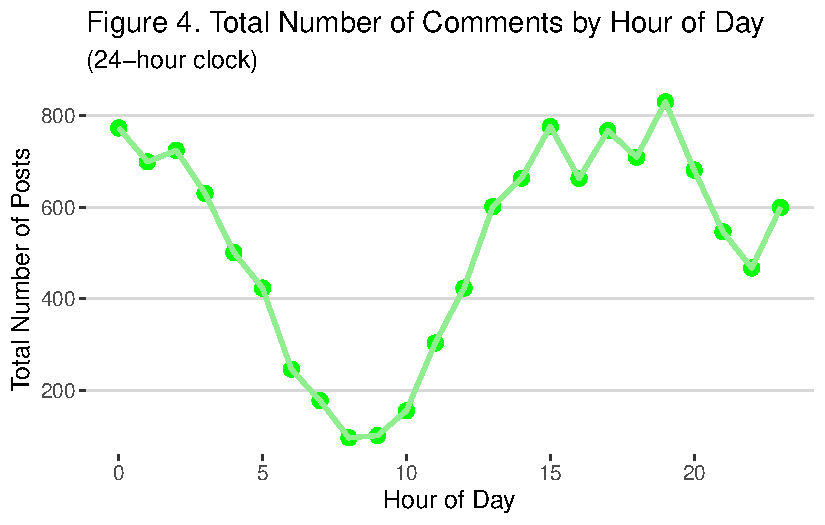
\includegraphics{paper_files/figure-pdf/unnamed-chunk-5-2.pdf}

\subsection{What are the words in the set of posts you have assembled
that appear most
frequently?}\label{what-are-the-words-in-the-set-of-posts-you-have-assembled-that-appear-most-frequently}

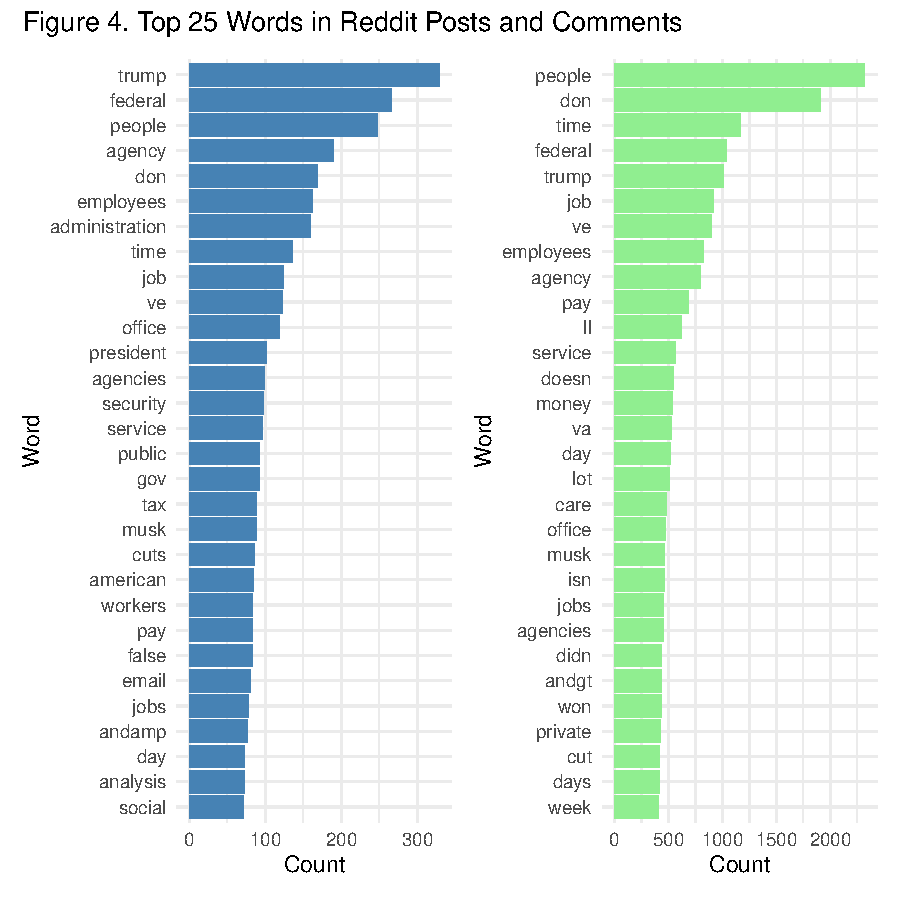
\includegraphics{paper_files/figure-pdf/unnamed-chunk-6-1.pdf}

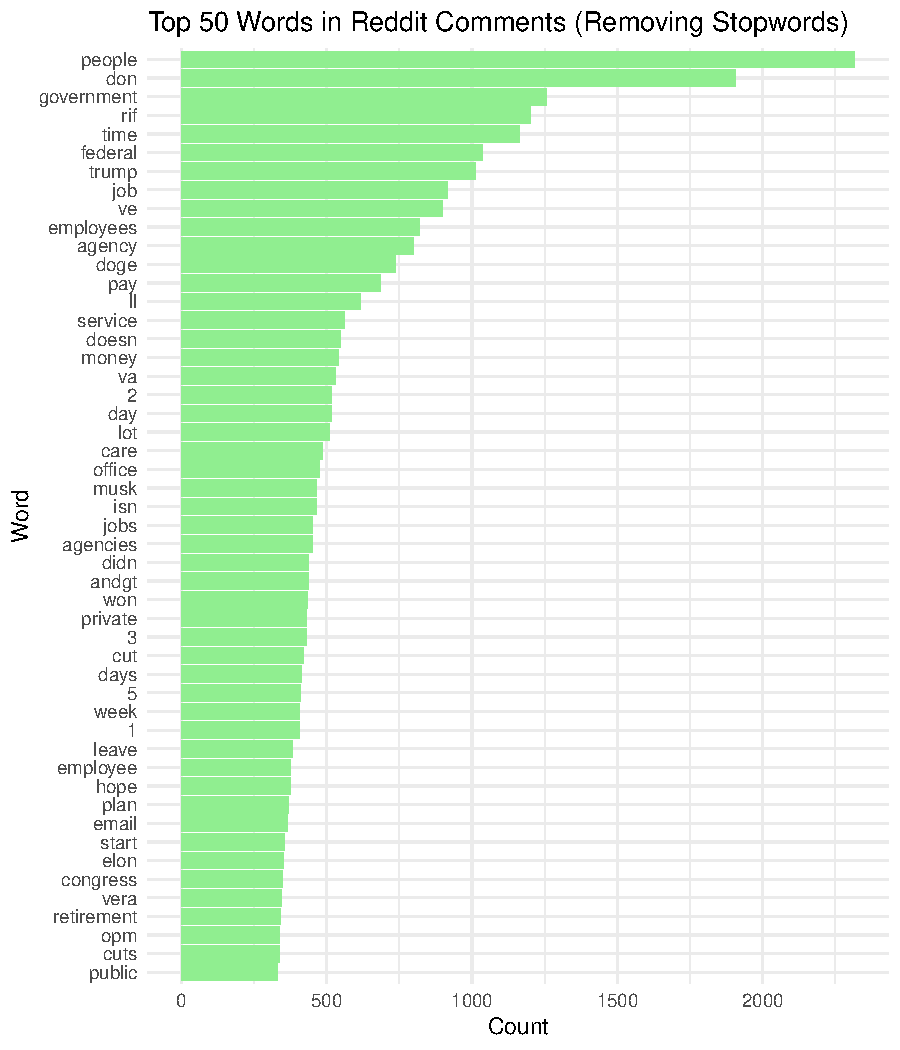
\includegraphics{paper_files/figure-pdf/unnamed-chunk-6-2.pdf}

The graphs above show the most frequent words in both Reddit posts and
their comments. However, many of these words are stopwords, which don't
provide much insight into the actual content of the discussions. To get
a better understanding of what people are really talking about, we will
remove these stopwords in the next step.

\subsection{How does this change if you exclude ``stop words'' such as
``a,'' ``an,'' ``the,'' ``is,'' and others that are common in English
sentences but are generally not
informative?}\label{how-does-this-change-if-you-exclude-stop-words-such-as-a-an-the-is-and-others-that-are-common-in-english-sentences-but-are-generally-not-informative}

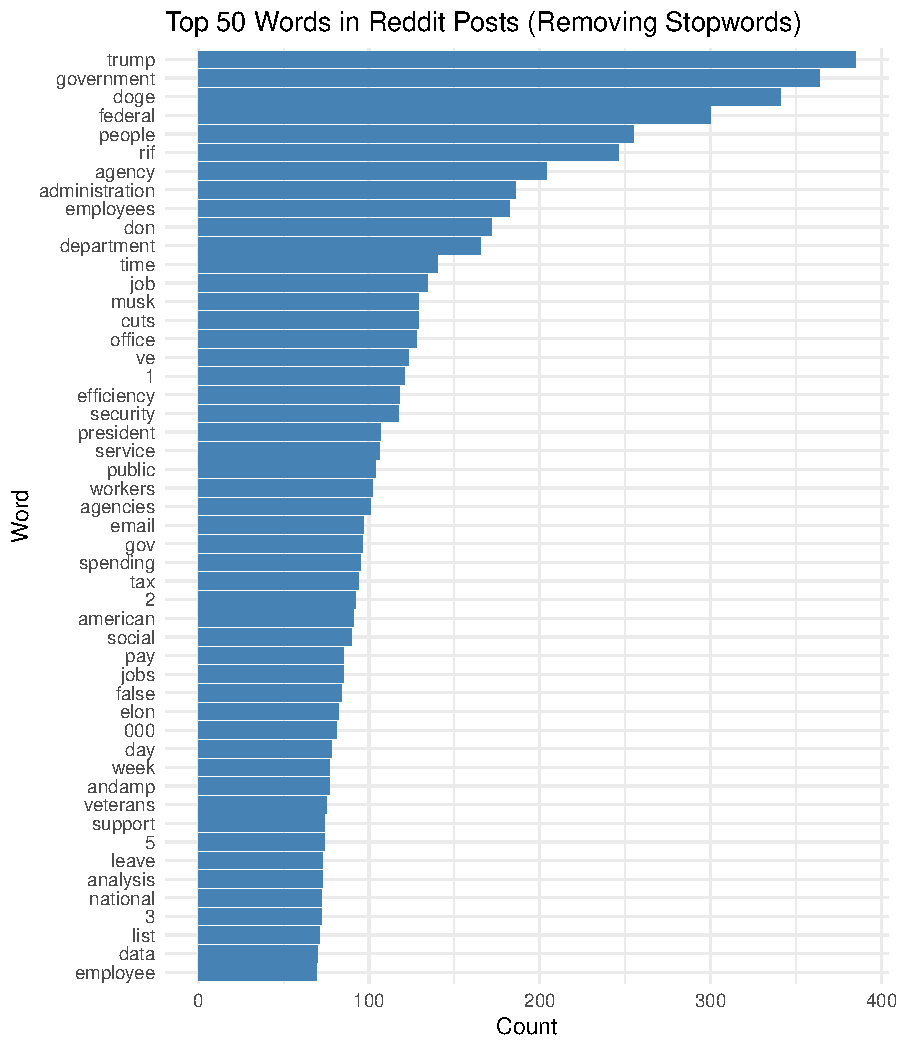
\includegraphics{paper_files/figure-pdf/unnamed-chunk-7-1.pdf}

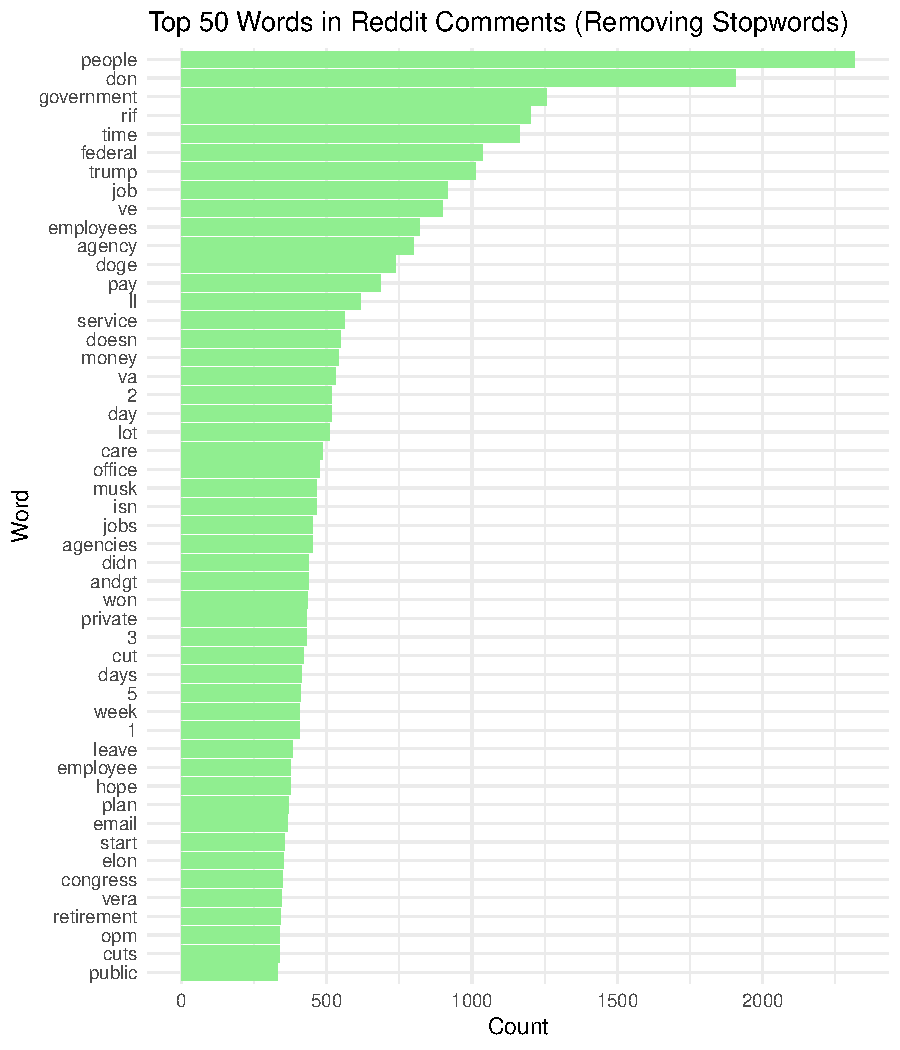
\includegraphics{paper_files/figure-pdf/unnamed-chunk-7-2.pdf}

The graphs above show the most frequent words used in both Reddit posts
and their comment sections. We can see that many of these words are
directly related to our topic, with frequent mentions of the President,
DOGE, the federal government, and RIF.

\emph{Coding Comments}. We coded 400 comments chosen at random

\begin{longtable}[]{@{}lr@{}}
\caption{Distribution of favorability coding for 400
comments}\tabularnewline
\toprule\noalign{}
outcome & Total \\
\midrule\noalign{}
\endfirsthead
\toprule\noalign{}
outcome & Total \\
\midrule\noalign{}
\endhead
\bottomrule\noalign{}
\endlastfoot
Not Coded & 12153 \\
favor & 110 \\
neutral & 73 \\
oppose & 217 \\
\end{longtable}

\newpage

\section{Appendix}\label{appendix}

\begin{longtable}[]{@{}l@{}}
\caption{List of subreddits relevant to the topic of
DOGE}\tabularnewline
\toprule\noalign{}
subreddit \\
\midrule\noalign{}
\endfirsthead
\toprule\noalign{}
subreddit \\
\midrule\noalign{}
\endhead
\bottomrule\noalign{}
\endlastfoot
50501 \\
fednews \\
neoliberal \\
FedEmployees \\
WhatTrumpHasDone \\
Whistleblowers \\
economy \\
PoliticalOpinions \\
Trumpvirus \\
Virginia \\
Libertarian \\
AskTrumpSupporters \\
Askpolitics \\
Conservative \\
VeteransAffairs \\
economicCollapse \\
feddiscussion \\
maryland \\
govfire \\
\end{longtable}




\end{document}
